\documentclass[aspectratio=169]{beamer}


\usepackage[utf8]{inputenc}
\usepackage{amsmath}
\usepackage{amsfonts}
\usepackage{amssymb}
\usepackage{graphicx}
\usepackage{ragged2e}  % `\justifying` text
\usepackage{booktabs}  % Tables
\usepackage{tabularx}
\usepackage{tikz}      % Diagrams
\usetikzlibrary{calc, shapes, backgrounds}
\usepackage{enumitem, amssymb}
\usepackage{pifont}
\usepackage{amsmath}
\usepackage{amssymb}
\usepackage{dsfont}
\usepackage{xr-hyper}
\usepackage{multirow}
\usepackage{url}       % `\url
\usepackage{pgfplots}
\usepackage[mode=buildnew]{standalone}
\usepackage{listings}  % Code listings
\usepackage[T1]{fontenc}
\externaldocument[M-]{models}[docs/models.tex]
\externaldocument[I-]{datsets}[docs/datasets.tex]

\usepackage{theme/beamerthemehbrs}


\newlist{todolist}{itemize}{2}
\setlist[todolist]{label=$\square$}
\newcommand{\cmark}{\ding{51}}%
\newcommand{\xmark}{\ding{55}}%
\newcommand{\done}{\rlap{$\square$}{\raisebox{2pt}{\large\hspace{1pt}\cmark}}%
\hspace{-2.5pt}}
\newcommand{\wontfix}{\rlap{$\square$}{\large\hspace{1pt}\xmark}}

\author[]{Lokesh Veeramacheneni}
\title{Out-of-distribution detection in 3D semantic segmentation models}
\subtitle{Master thesis}
\institute[HBRS]{Hochschule Bonn-Rhein-Sieg}
\date{September 10, 2021}
\subject{Test beamer}
\thirdpartylogo{theme/images/DFKI.png}


\begin{document}
{
\begin{frame}
\titlepage
\end{frame}
}
\begin{frame}{Topics}
    \begin{itemize}
        \item[1.] Out of distribution (OOD)/Anomaly/Distributional shift
        \item[2.] Dataset study
        \item[3.] Model study
    \end{itemize}
\end{frame}

\begin{frame}{OOD/Anomaly/Distributional shift}
    \begin{itemize}
        \item[$\bullet$] \textbf{Anomaly} - Patterns that do not conform to the expected behaviour in the training
        data
        \item[$\bullet$] \textbf{OOD} - The test input is drawn from an unknown distribution of unknown data
        which is far from the training distribution
        \item[$\bullet$] \textbf{Distributional Shift} - The input to the model is a slightly shifted version of training data distribution
    \end{itemize}
    %As an example, let us assume
    %\begin{itemize}
    %    \item[$\bullet$] Universal dataset - Imagenet (10000 classes)
    %    \item[$\bullet$] Train and test dataset - CIFAR-10 (10 classes) \newline (Airplane, Automobile, Bird, Cat, Deer, Dog, $Frog^{*}$, Horse, Ship, Truck)
    %\end{itemize}
    
\end{frame}

\begin{frame}{OOD/Anomaly/Distributional shift}
    \begin{figure}
        \centering
        \caption{Images showing the distributional shift in data, anomalies and OOD data using ship example. Images taken from [1], [2], [3], [4], [5] and [6].}
        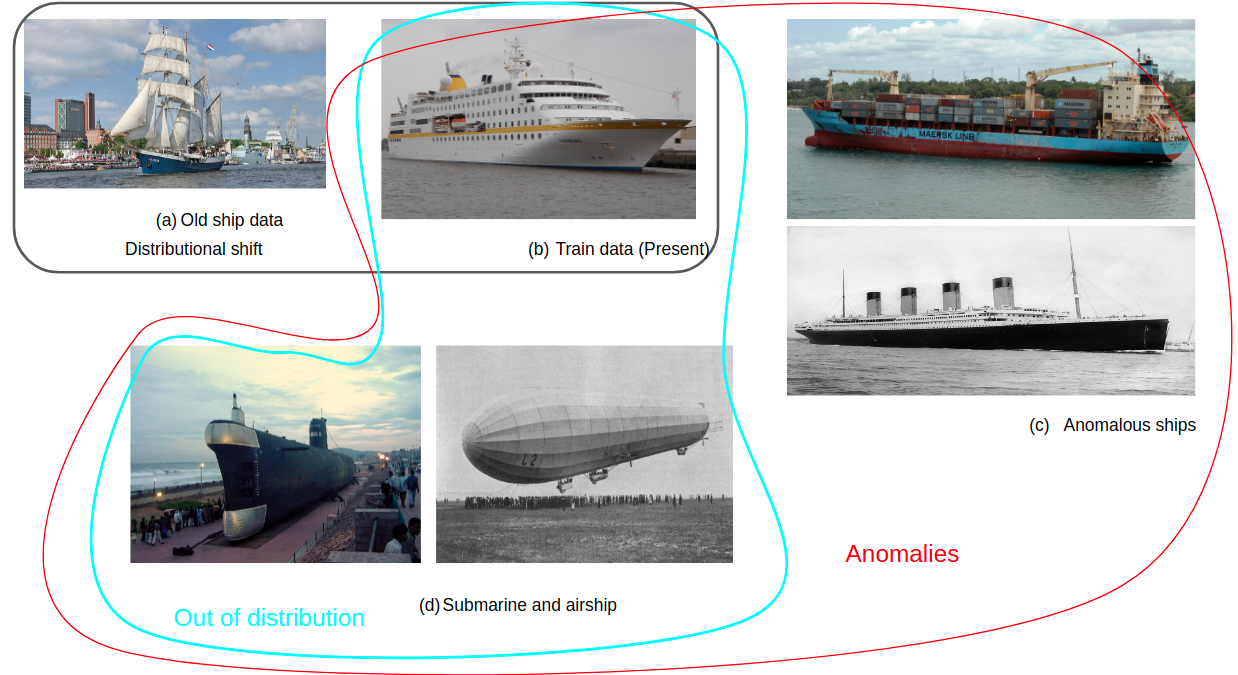
\includegraphics[scale=0.25]{ships.png}
    \end{figure}
\end{frame}

\begin{frame}{Datasets survey}
    % \resizebox{\textwidth}{0.25\textheight}{%
    % % \begin{table}[]
    % %\centering
    % % \caption{3D LiDAR datasets classified based on the acquisition type. Table updated from \cite{survey3d}}
    % \begin{tabular}{c|c|c|c|c|c}%|c}
    %     \hline
    %     % acquisition type, dataset, frames, #points, classes, I/O, year
    %     acquisition mode & dataset & frames & points (in million) & classes & scene type \\  % & pub. year \\
    %     \hline
    %     \multirow{7}{*}{static} & Oakland & 17 & 1.6 &  44 & outdoor \\ % & 2009 \\ 
    %                             & Paris-lille-3D & 3 & 143 & 50 & outdoor \\ % & 2018 \\
    %                             & Paris-rue-Madame & 2 & 20 & 17 & outdoor \\ %& 2014 \\
    %                             & S3DIS& 5 & 215 & 12 & indoor \\ %& 2016 \\
    %                             & ScanObjectNN & - & - & 15 & indoor \\ %& 2019 \\
    %                             & Semantic3D & 30 & 4009 & 8 & outdoor \\ %& 2017 \\
    %                             & TerraMobilita/IQmulus & 10 & 12 & 15 & outdoor\\ % & 2015 \\
    %                             & TUM City Campus & 631 & 41 & 8 & outdoor\\ % & 2016 \\
    %                             & DALES & 40 (tiles) & 492 & 8 & outdoor\\ % & 2021\\
    %     \hline
    %     \multirow{7}{*}{sequential} & A2D2 & 41277 & 1238 & 38 & outdoor\\ % & 2020\\
    %                                 & AIO Drive & 100& - & 23 & outdoor\\ % & 2020\\
    %                                 & KITTI-360 & 100K & 18000 & 19 & outdoor\\ %& 2020\\
    %                                 & nuScenes-lidarseg & 40000 & 1400 & 32& outdoor\\ % & 2020\\
    %                                 & PandaSet & 16000 & 1844 & 37 & outdoor \\ %& 2020\\
    %                                 & SemanticKITTI & 43552 & 4549 & 28 & outdoor \\ %& 2019\\
    %                                 & SemanticPOSS & 2988 & 216 & 14 & outdoor \\ %& 2020\\
    %                                 & Sydney Urban & 631 & - & 26 & outdoor\\ % & 2013\\
    %                                 & Toronto-3D & 4 & 78.3& 8& outdoor\\ % & 2020\\

    %     \hline
    %     \multirow{1}{*}{synthetic}  & SynthCity & 75000 & 367.9 & 9 & outdoor \\ %& 2019\\
    %     \hline
    % \end{tabular}
    % \caption{hjsadvfjdf}
    % \label{table:3d_lidar_datasets_table}
% }
    % \end{table}
    \begin{figure}
        \centering
        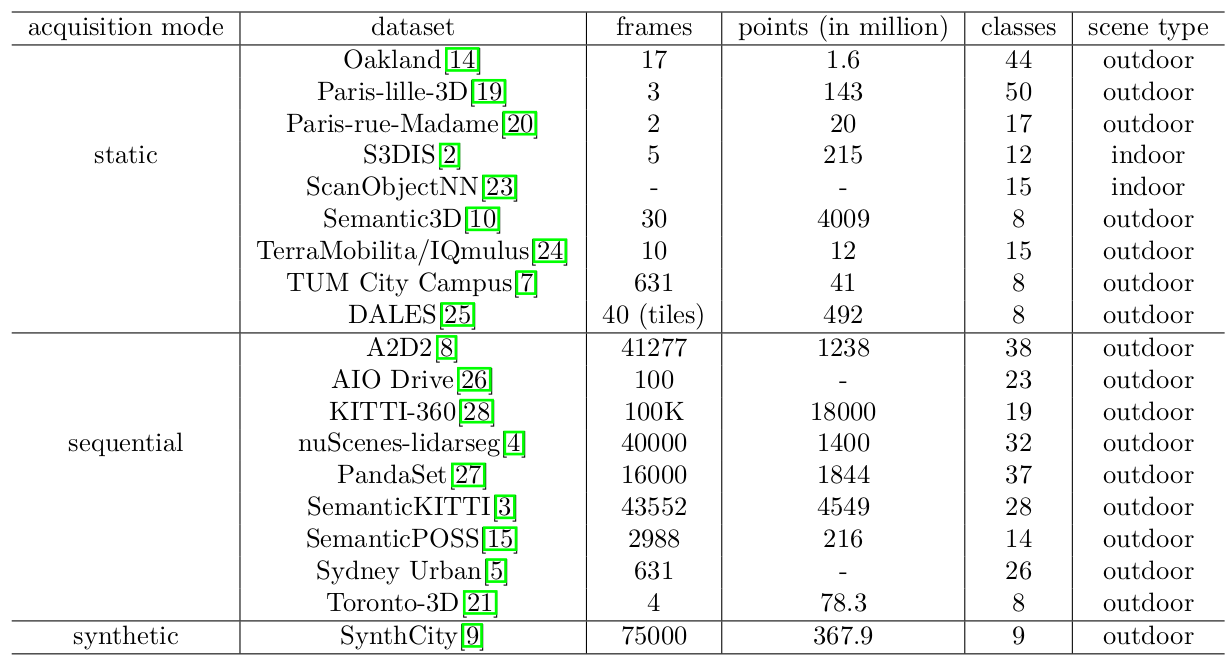
\includegraphics[width=0.75\textwidth]{datasets.png}
        \caption{Surveyed datasets for the 3D LiDAR data.}
       
    \end{figure}
\end{frame}

\begin{frame}{Semantic3D Vs SemanticKITTI}
    %\begin{column}{0.5\textwidth}
    \begin{itemize}
        \item[1.] Both are widely evaluated and have highest number of points
        \item[2.] Both are part of benchmark challenge
        \item[3.] Synthetic datasets cannot be used for training, they lack the accuracy in detail
        \item[4.] SemanticKITTI has 3D coordinates and intensity as features
        \item[5.] In addition to 3D coordinates and intensity, Semantic3D also has RGB
        \item[6.] Semantic3D is more diverse rather than SemanticKITTI dataset
    \end{itemize}
    %\end{column}
    %\begin{column}{0.5\textwidth}
    %\begin{figure}
    %    \centering
    %    \includegraphics[scale=0.195]{theme/images/diversity.png}
    %    \caption{Confusion matrix of diversity distance to measure the diversity between scenes in a dataset and also cross dataset. Image taken from \cite{9430028}}
    %    \label{fig:my_label}
    %\end{figure}
    %\end{column}

\end{frame}

\begin{frame}{Training dataset - Semantic3D}
\begin{columns}
    \begin{column}{0.5\textwidth}
    \begin{itemize}
        \item[1.] Large set of points ($\approx$ 4 million)
        \item[2.] Eight semantic classes
        \item[3.] Comes with 3D coordinates, RGB and intensity as features
        \item[4.] Well studied and benchmarked dataset
        \item[5.] Include variety of urban and rural scenes of various complexity
        \item[6.] Dense point clouds with little overlap
    \end{itemize}
    \end{column}
    \begin{column}{0.5\textwidth}
    \begin{figure}
        \centering
        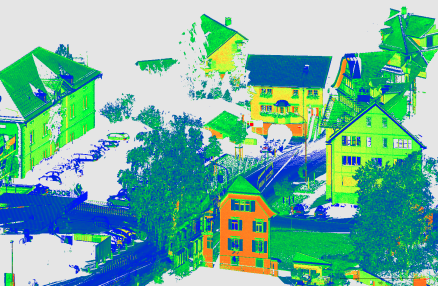
\includegraphics[scale=0.48]{sem3d.png}
        \caption{Example of a scene in semantic3D dataset}
       
    \end{figure}
    \end{column}
\end{columns}
    
\end{frame}


\begin{frame}{Models survey}
    \begin{itemize}
        \item[$\bullet$] RandLA-Net has shown higher performance with lower parameters - lower training time
    \end{itemize}
    \begin{figure}
        \centering
        % \includegraphics[scale=0.16]{theme/images/models_new.png}
        \includestandalone[width=0.45\linewidth]{models_plot}
        \caption{Models performance on SemanticKITTI plotted against the number of parameters}       
    \end{figure}
\end{frame}

\begin{frame}{Network - RandLA-Net}
    \begin{itemize}
        \item[1.] RandLA-Net employs random point sampling - lower preprocessing time
        \item[2.] RandLA-Net also uses Dilated residual block - scalable receptive field of a point
        \item[3.] RandLA-Net also uses attentive pooling - weighted features - Can employ OOD methods such as ODIN
    \end{itemize}
    \begin{figure}
        \centering
        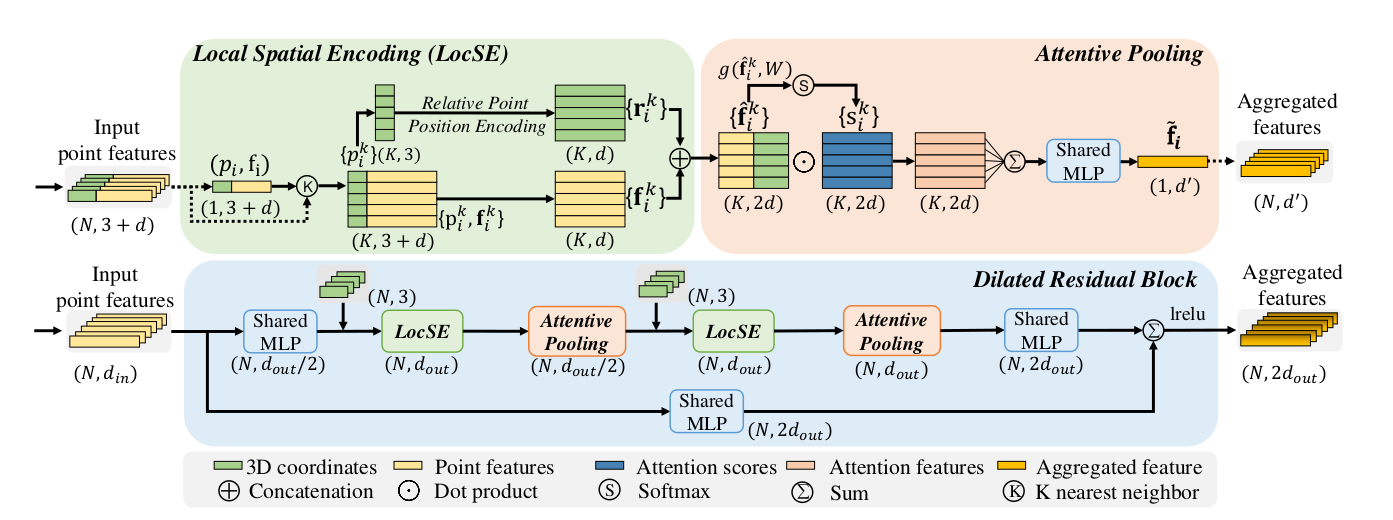
\includegraphics[scale=0.23]{Screenshot from 2021-11-18 01-36-34.png}
        \caption{Dilated residual block of RandLA-Net in below image along with subblocks of local spatial encoding and attentive pooling. Image from }
        
    \end{figure}
\end{frame}
% \section{First section}
% \subsection{A subsection}

% \begin{frame}{Jabberwocky}
%       \framesubtitle{Lewis Carroll}%
%       \begin{tikzpicture}[overlay,remember picture]
%         \node[anchor=south east,xshift=-30pt,yshift=35pt]
%           at (current page.south east) {
%             %\includegraphics[width=35mm]{resources/jabberwocky-light}
%           };
%       \end{tikzpicture}%
%       'Twas brillig, and the slithy toves\\
%       Did gyre and gimble in the wabe;\\
%       All mimsy were the borogoves,\\
%       And the mome raths outgrabe.\\\bigskip

%       “Beware the Jabberwock, my son!\\
%       The jaws that bite, the claws that catch!\\
%       Beware the Jubjub bird, and shun\\
%       The frumious Bandersnatch!”\\
% \end{frame}


% \begin{frame}[label=lists]{Lists and locales}
%       \framesubtitle{Lorem ipsum dolor sit amet}
%       \begin{columns}[onlytextwidth]
%         \column{.5\textwidth}
%           \begin{itemize}
%             \item Nulla nec lacinia odio. Curabitur urna tellus.
%             \begin{itemize}
%               \item Fusce id sodales dolor. Sed id metus dui.
%               \begin{itemize}
%                 \item Cupio virtus licet mi vel feugiat.
%               \end{itemize}
%             \end{itemize}
%           \end{itemize}
%         \column{.5\textwidth}
%           \begin{enumerate}
%             \item Donec porta, risus porttitor egestas scelerisque video.
%             \begin{enumerate}
%               \item Nunc non ante fringilla, manus potentis cario.
%               \begin{enumerate}
%                 \item Pellentesque servus morbi tristique.
%               \end{enumerate}
%             \end{enumerate}
%           \end{enumerate}
%       \end{columns}
%       \bigskip
%       \justifying

%       {\uselanguage{czech}Nechť již hříšné saxofony ďáblů
%       rozzvučí síň úděsnými tóny waltzu, tanga a quickstepu!}
%       {\uselanguage{slovak} Nezvyčajné kŕdle šťastných figliarskych
%       ďatľov učia pri kótovanom ústí Váhu mĺkveho koňa Waldemara
%       obžierať väč\-šie kusy exkluzívnej kôry.}
%       {\uselanguage{english}The quick, brown fox jumps over a lazy
%       dog. DJs flock by when MTV ax quiz prog. “Now fax quiz Jack!”}
% \end{frame}

% \subsection{Structuring Elements}
%     \begin{frame}[label=simmonshall]{Text blocks}
%       \framesubtitle{In plain, example, and \alert{alert} flavour}
%       \alert{This text} is highlighted.

%       \begin{block}{A plain block}
%         This is a plain block containing some \alert{highlighted text}.
%       \end{block}
%       \begin{exampleblock}{An example block}
%         This is an example block containing some \alert{highlighted text}.
%       \end{exampleblock}
%       \begin{alertblock}{An alert block}
%         This is an alert block containing some \alert{highlighted text}.
%       \end{alertblock}
%     \end{frame}


% \begin{frame}[label=proof]{Definitions, theorems, and proofs}
%       \framesubtitle{All integers divide zero}
%       \begin{definition}
%         $\forall a,b\in\mathds{Z}: a\mid b\iff\exists c\in\mathds{Z}:a\cdot c=b$
%       \end{definition}
%       \begin{theorem}
%         $\forall a\in\mathds{Z}: a\mid 0$
%       \end{theorem}
%       \begin{proof}[Proof\nopunct]
%       	$\forall a\in \mathds{Z}:\cdot 0=0$
%       \end{proof}
% \end{frame}

%     \subsection{Numerals and Mathematics}
%     \begin{frame}[label=math]{Numerals and Mathematics}
%       \framesubtitle{Formulae, equations, and expressions}
%       \begin{columns}[onlytextwidth]
%         \column{.20\textwidth}
%           1234567890
%         \column{.20\textwidth}
%           \oldstylenums{1234567890}
%         \column{.20\textwidth}
%           $\hat{x}$, $\check{x}$, $\tilde{a}$,
%          $\bar{a}$, $\dot{y}$, $\ddot{y}$
%         \column{.40\textwidth}
%           $\int \!\! \int f(x,y,z)\,\mathsf{d}x\mathsf{d}y\mathsf{d}z$
%       \end{columns}
%       \begin{columns}[onlytextwidth]
%         \column{.5\textwidth}
%           $$\frac{1}{\displaystyle 1+
%             \frac{1}{\displaystyle 2+
%             \frac{1}{\displaystyle 3+x}}} +
%             \frac{1}{1+\frac{1}{2+\frac{1}{3+x}}}$$
%         \column{.5\textwidth}
%           $$F:\left| \begin{array}{ccc}
%           F''_{xx} & F''_{xy} &  F'_x \\
%           F''_{yx} & F''_{yy} &  F'_y \\
%           F'_x     & F'_y     & 0
%          \end{array}\right| = 0$$
%       \end{columns}
%       \begin{columns}[onlytextwidth]
%         \column{.3\textwidth}
%           $$\mathop{\int \!\!\! \int}_{\mathbf{x} \in \mathds{R}^2}
%           \! \langle \mathbf{x},\mathbf{y}\rangle\,\mathsf{d}\mathbf{x}$$
%         \column{.33\textwidth}
%          $$\overline{\overline{a\alpha}^2+\underline{b\beta}
%           +\overline{\overline{d\delta}}}$$
%         \column{.37\textwidth}
%           $\left] 0,1\right[ + \lceil x \rfloor - \langle x,y\rangle$
%       \end{columns}
%       \begin{columns}[onlytextwidth]
%         \column{.4\textwidth}
%           \begin{eqnarray*}
%           e^x &\approx& 1+x+x^2/2! + \\
%              && {}+x^3/3! + x^4/4!
%           \end{eqnarray*}
%         \column{.6\textwidth}
%           $${n+1\choose k} = {n\choose k} + {n \choose k-1}$$
%       \end{columns}
%     \end{frame}

%     \subsection{Figures and Code Listings}
%     \begin{frame}[label=figs1]{Figures}
%       \framesubtitle{Tables, graphs, and images}
%       \begin{table}[!b]
% %        {\carlitoTLF % Use monospaced lining figures
%         \begin{tabularx}{\textwidth}{Xrrr}
%           \textbf{Faculty} & \textbf{With \TeX} & \textbf{Total} &
%           \textbf{\%} \\
%           \toprule
%           Faculty of Informatics       & 1\,716  & 2\,904  &
%           59.09 \\% 1433
%           Faculty of Science           & 786     & 5\,275  &
%           14.90 \\% 1431
%           Faculty of $\genfrac{}{}{0pt}{}{\textsf{Economics and}}{%
%           \textsf{Administration}}$    & 64      & 4\,591  &
%           1.39  \\% 1456
%           Faculty of Arts              & 69      & 10\,000 &
%           0.69  \\% 1421
%           Faculty of Medicine          & 8       & 2\,014  &
%           0.40  \\% 1411
%           Faculty of Law               & 15      & 4\,824  &
%           0.31  \\% 1422
%           Faculty of Education         & 19      & 8\,219  &
%           0.23  \\% 1441
%           Faculty of Social Studies    & 12      & 5\,599  &
%           0.21  \\% 1423
%           Faculty of Sports Studies    & 3       & 2\,062  &
%           0.15  \\% 1451
%           \bottomrule
%         \end{tabularx}%}
%         \caption{The distribution of theses written using \TeX\ during 2010--15 at MU}
%       \end{table}
%     \end{frame}
%     \begin{frame}[label=figs2]{Figures}
%       \framesubtitle{Tables, graphs, and images}
%       \begin{figure}[b]
%         \centering
%         % Flipping a coin
%         % Author: cis
%         \tikzset{
%           head/.style = {fill = none, label = center:\textsf{H}},
%           tail/.style = {fill = none, label = center:\textsf{T}}}
%         \scalebox{0.65}{\begin{tikzpicture}[
%             scale = 1.5, transform shape, thick,
%             every node/.style = {draw, circle, minimum size = 10mm},
%             grow = down,  % alignment of characters
%             level 1/.style = {sibling distance=3cm},
%             level 2/.style = {sibling distance=4cm},
%             level 3/.style = {sibling distance=2cm},
%             level distance = 1.25cm
%           ]
%           \node[shape = rectangle,
%             minimum width = 6cm, font = \sffamily] {Coin flipping}
%           child { node[shape = circle split, draw, line width = 1pt,
%                   minimum size = 10mm, inner sep = 0mm, rotate = 30] (Start)
%                   { \rotatebox{-30}{H} \nodepart{lower} \rotatebox{-30}{T}}
%           child {   node [head] (A) {}
%              child { node [head] (B) {}}
%              child { node [tail] (C) {}}
%           }
%           child {   node [tail] (D) {}
%              child { node [head] (E) {}}
%              child { node [tail] (F) {}}
%           }
%           };

%           % Filling the root (Start)
%           \begin{scope}[on background layer, rotate=30]
%             \fill[head] (Start.base) ([xshift = 0mm]Start.east) arc (0:180:5mm)
%               -- cycle;
%             \fill[tail] (Start.base) ([xshift = 0pt]Start.west) arc (180:360:5mm)
%               -- cycle;
%           \end{scope}

%           % Labels
%           \begin{scope}[nodes = {draw = none}]
%             \path (Start) -- (A) node [near start, left]  {$0.5$};
%             \path (A)     -- (B) node [near start, left]  {$0.5$};
%             \path (A)     -- (C) node [near start, right] {$0.5$};
%             \path (Start) -- (D) node [near start, right] {$0.5$};
%             \path (D)     -- (E) node [near start, left]  {$0.5$};
%             \path (D)     -- (F) node [near start, right] {$0.5$};
%             \begin{scope}[nodes = {below = 11pt}]
%               \node [name = X] at (B) {$0.25$};
%               \node            at (C) {$0.25$};
%               \node [name = Y] at (E) {$0.25$};
%               \node            at (F) {$0.25$};
%             \end{scope}
%           \end{scope}
%         \end{tikzpicture}}
%         \caption{Tree of probabilities -- Flipping a coin\footnote[frame]{%
%           A derivative of a diagram from \url{texample.net} by cis, CC BY 2.5 licensed}}
%       \end{figure}
%     \end{frame}

%     \defverbatim[colored]\sleepSort{
%       \begin{lstlisting}[language=C,tabsize=2]
%   #include <stdio.h>
%   #include <unistd.h>
%   #include <sys/types.h>
%   #include <sys/wait.h>

%   // This is a comment
%   int main(int argc, char **argv)
%   {
%           while (--c > 1 && !fork());
%           sleep(c = atoi(v[c]));
%           printf("%d\n", c);
%           wait(0);
%           return 0;
%   }
%     \end{lstlisting}}
%     \begin{frame}{Code listings}{An example source code in C}
%       \sleepSort
%     \end{frame}

%     \subsection{Citations and Bibliography}
%     \begin{frame}[label=citations]{Citations}
%       \framesubtitle{\TeX, \LaTeX, and Beamer}

%       \justifying\TeX\ is a programming language for the typesetting
%       of documents. It was created by Donald Erwin Knuth in the late
%       1970s and it is documented in \emph{The \TeX
%       book}~\cite{knuth84}.

%       In the early 1980s, Leslie Lamport created the initial version
%       of \LaTeX, a high-level language on top of \TeX, which is
%       documented in \emph{\LaTeX : A Document Preparation
%       System}~\cite{lamport94}. There exists a healthy ecosystem of
%       packages that extend the base functionality of \LaTeX;
%       \emph{The \LaTeX\ Companion}~\cite{MG94} acts as a guide
%       through the ecosystem.

%       In 2003, Till Tantau created the initial version of Beamer, a
%       \LaTeX\ package for the creation of presentations. Beamer is
%       documented in the \emph{User's Guide to the Beamer
%       Class}~\cite{tantau04}.
%     \end{frame}

%     \begin{frame}[label=bibliography]{Bibliography}
%       \framesubtitle{\TeX, \LaTeX, and Beamer}
%       \begin{thebibliography}{9}
%         \bibitem{knuth84}
%             Donald~E.~Knuth.
%             \emph{The \TeX book}.
%             Addison-Wesley, 1984.
%         \bibitem{lamport94}
%             Leslie~Lamport.
%             \emph{\LaTeX : A Document Preparation System}.
%             Addison-Wesley, 1986.
%         \bibitem{MG94}
%             M.~Goossens, F.~Mittelbach, and A.~Samarin.
%             \emph{The \LaTeX\ Companion}.
%             Addison-Wesley, 1994.
%         \bibitem{tantau04}
%             Till~Tantau.
%             \emph{User's Guide to the Beamer Class Version 3.01}.
%             Available at \url{http://latex-beamer.sourceforge.net}.
%         \bibitem{MS05}
%             A.~Mertz and W.~Slough.
%             Edited by B.~Beeton and K.~Berry.
%             \emph{Beamer by example} In TUGboat,
%               Vol. 26, No. 1., pp. 68-73.
%       \end{thebibliography}
%     \end{frame}


% \section{Something else}

% \begin{frame}
% \frametitle{There Is No Largest Prime Number}
% \framesubtitle{The proof uses \textit{reductio ad absurdum}.}
% \begin{theorem}
% There is no largest prime number. \end{theorem}
% \begin{enumerate}
% \item<1-| alert@1> Suppose $p$ were the largest prime number.
% \item<2-> Let $q$ be the product of the first $p$ numbers.
% \item<3-> Then $q+1$ is not divisible by any of them.
% \item<1-> But $q + 1$ is greater than $1$, thus divisible by some prime
% number not in the first $p$ numbers.
% \end{enumerate}
% \end{frame}

% \begin{frame}{A longer title}
% \begin{itemize}
% \item one
% \item two

% \textbf{This is a test of bold text}

% \end{itemize}
% \end{frame}

% \begin{frame}[allowframebreaks]{Test}
%   First slide
%   \begin{itemize}
%     \item
%     \item
%     \item
%     \item
%     \item
%   \end{itemize}
%   \framebreak
%   Second slide
%   \begin{itemize}
%     \item
%     \item
%     \item
%     \item
%     \item
%   \end{itemize}
% \end{frame}
% %--- Next Frame ---%



\end{document}
